\documentclass[../main.tex]{subfiles}

\begin{document}
\section{详细设计}

% 说明,包括:
% 接口描述
% 功能描述
% 所用数据结构说明
% 算法描述

% main4.tex 暂时更完了,最后再往里面加图————话说你们有矢量图(指word里面的那些图)嘛,没有的话我看怎么自己处理一下

% 一个图片引用的示例
% \begin{figure}[ht]
% \centering
% 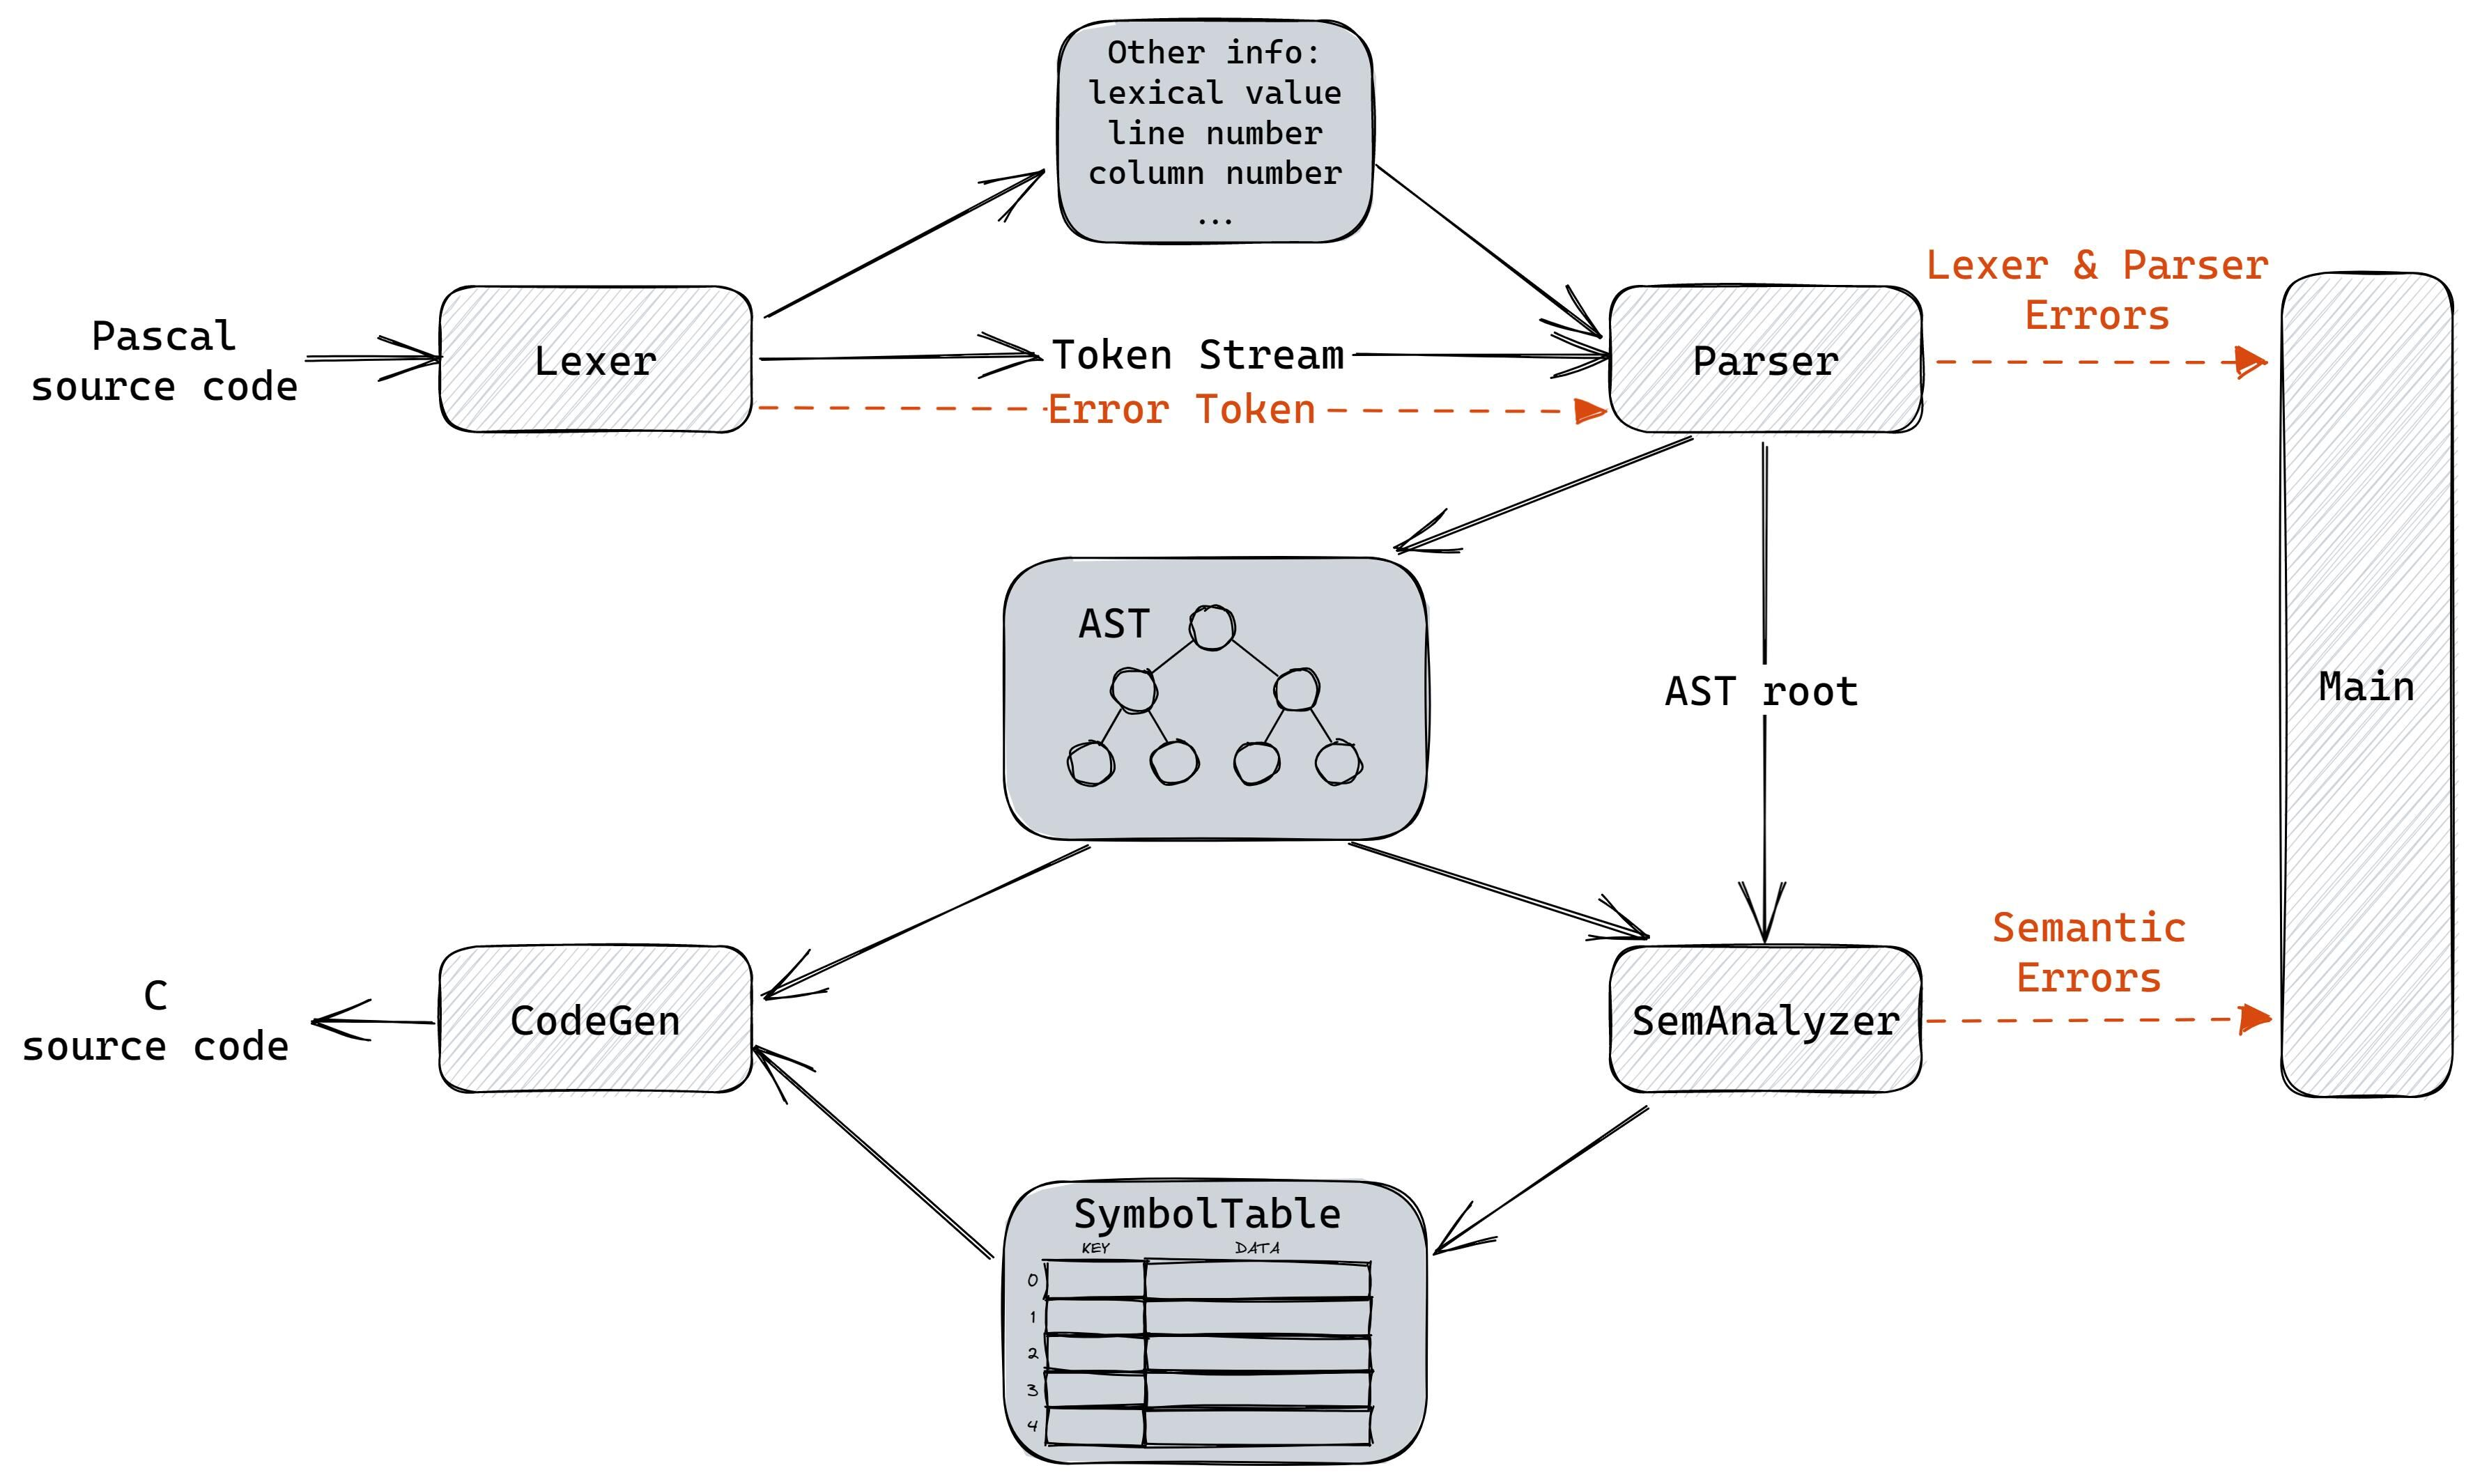
\includegraphics[width=\linewidth]{assets/1.jpg}
% \caption{非终结符的First集合计算示例}
% \label{fig:first_set}
% \end{figure}

% 备注一下,本部分的图片等资源暂未上传

\subsection{词法分析}

词法分析器由以下类构成:
\begin{itemize}
\item 词法分析器主体 - Lexer
    \begin{itemize}
        \item 保存词法元素(关键字、分隔符等)
        \item 给予词法状态机输入,将获得的Token添加到输出列表
    \end{itemize}
\item 构造记号的工厂 - TokenFactory
    \begin{itemize}
        \item 构造并返回不同的记号类
    \end{itemize}
\item 翻译表产生的判断规则 - LexRules
    \begin{itemize}
        \item 提供判断字符类型的方法
    \end{itemize}
\end{itemize}

\subsubsection{功能}

对于一些能在词法分析阶段完成的工作,将尽可能提前完成,如:
\begin{itemize}
\item 对十六进制数字的字面量进行修改,将“\$”修改为C风格的“0x”;
\item 判断数值类型,划分为Real,Hex,Integer;
\item 对“.”符号进行细化,区分为Dot和Period;
\item 避免大小写对后阶段分析的干扰,将关键字等类别转化为Enum类型;
\end{itemize}

此外,对注释可以识别以下三种:
\begin{itemize}
\item {……}
\item (*……*)
\item //
\end{itemize}

\texttt{Lexer} 是接口\texttt{ILexer}的实现类,其的功能包括:
\begin{itemize}
    \item 注释处理:识别并跳过源代码中的注释。
    \item 词法记号生成:根据源代码生成相应的词法记号,包括关键字、标识符、数值、运算符、分隔符等。
    \item 错误处理:在源代码中识别非法字符和格式错误,并抛出错误信息。
\end{itemize}

\subsubsection{数据结构及内部算法}

\paragraph{LexemeFactory}
采用工厂模式,提供了静态的多态的方法 \texttt{MakeToken} 来创建不同类型的词法记号。

\begin{lstlisting}[
    style=csharp
]
public static SemanticToken MakeToken(SemanticTokenType tokenType, 
                                      string literal, uint _line, uint _chPos)
{
    /* 实际的逻辑代码 */
}
\end{lstlisting}

\paragraph{LexRules}
\texttt{LexRules} 包含了各种词法规则的静态方法,用于判断字符是否为字母、数字、运算符等。此外,它还为关键字、分隔符和操作符提供了字符串数组来记录内容,这些内容可根据语法分析进行调整或进一步拓展。这些方法非常重要,因为它们确保词法分析器可以正确地识别各种词法元素,从而为语法分析阶段准备正确的输入。该类的中的函数有:
\begin{itemize}
    \item \textbf{IsKeyword}: 判断一个字符串是否为预定义的关键字。这有助于词法分析器正确区分标识符和保留关键字。它能将大小写字母看作同一字符进行比较,确保Pascal转C语言的语法正确性。
    \item \textbf{IsDelimiter}: 判断字符是否为词法单元的分隔符。
    \item \textbf{IsOperator}: 判断字符是否为运算符,支持词法分析的运算符识别。
    \item \textbf{IsDigit}: 判断字符是否为数字,用于识别数值。
    \item \textbf{IsHexDigit}: 判断字符是否为十六进制数的有效字符。
    \item \textbf{IsLetter}: 判断字符是否为字母或下划线,这对于识别标识符尤其重要。
\end{itemize}

\paragraph{Lexer} 词法分析器\texttt{Lexer}的核心是一个以状态机为基础的类,用于根据输入文本的不同部分切换状态,识别和生成不同的词法记号。以下是状态机可能进入的状态,使用枚举类型实现:

\begin{lstlisting}[
    style=csharp
]
public enum StateType
{
    Start,      // 初始状态,用于开始分析新的token
    Comment,    // 处理注释的状态
    Word,       // 处理单词(关键字或标识符)
    Num,        // 处理数字(整数或浮点数)
    Delimiter,  // 处理分隔符
    Operator,   // 处理操作符
    Unknown,    // 遇到未知字符或字符串
    Done        // 完成所有分析
}
\end{lstlisting}

\texttt{Tokenize()} 函数是状态机的主要工作函数,负责根据当前状态来处理输入的源代码字符串,并进行状态转移,直到读取完整个字符串。最终,它将返回一个词法记号流 (\texttt{\_tokens})。词法记号的字面量通过 \texttt{StringBuilder} 类记录。

\begin{lstlisting}[
    style=csharp
]
public List<SemanticToken> Tokenize()
{
    while (_state != StateType.Done)  // 当状态不是“完成”时,继续处理输入
    {
        switch (_state)
        {
            case StateType.Start:
                HandleStartState();  // 处理起始状态
                break;
            case StateType.Comment:
                // 根据注释的类型调用不同的处理函数
                if (_ch == '{')
                {
                    HandleCommentStateBig();
                }
                else if (_ch == '*')
                {
                    HandleCommentStateSmall();
                }
                else
                {
                    HandleCommentSingleLine();
                }
                break;
            case StateType.Num:
                HandleNumState();  // 处理数值状态
                break;
            case StateType.Word:
                HandleWordState();  // 处理单词状态
                break;
            case StateType.Delimiter:
                HandleDelimiterState();  // 处理界符状态
                break;
            case StateType.Operator:
                HandleOperatorState();  // 处理操作符状态
                break;
            case StateType.Unknown:
                // 抛出未知词法元素异常
                throw new LexemeException(LexemeErrorType.UnknownCharacterOrString, _line, _chPos, "Illegal lexeme.");
            case StateType.Done:
                break;  // 完成所有处理,退出循环
        }
    }
    return _tokens;  // 返回生成的词法记号流
}
\end{lstlisting}

\texttt{HandleStartState()} 函数是词法分析器中首个调用的函数,负责从源代码中读取字符并确定其对应的状态。函数首先检查是否达到输入字符串的结尾,然后根据字符决定下一状态。此函数是实现词法分析的状态机逻辑的关键入口点,其设计考虑了各种字符输入可能性并做出相应状态转换。以下是该函数的详细解释与实现:

\begin{lstlisting}[
    style=csharp
]
private void HandleStartState()
{
    ResetTokenBuilder();  // 重置token构建器,准备构建新的token

    GetChar();  // 读取下一个字符
    GetNbc();   // 忽略空白字符
    if (_finish)  // 检查是否已经处理完所有输入
    {
        _state = StateType.Done;  // 设置状态为完成
        return;
    }

    // 根据读取的字符,判断进入哪个状态
    if (_ch == '{')  // 处理以 "{" 开始的注释
    {
        _state = StateType.Comment;
    }
    else if (_ch == '(')  // 处理以 "(" 开始可能是注释的情况
    {
        char nextChar = PeekNextChar();
        if (nextChar == '*')
        {
            GetChar();  // 消费 "*"
            _state = StateType.Comment;
        }
        else
        {
            _state = StateType.Delimiter;
        }
    }
    else if (_ch == '/')  // 处理以 "/" 开始可能是注释或运算符的情况
    {
        char nextChar = PeekNextChar();
        if (nextChar == '/')
        {
            GetChar();  // 消费第二个 "/"
            _state = StateType.Comment;
        }
        else
        {
            _state = StateType.Operator;
        }
    }
    else if (_ch == '.')  // 处理点号,可能是小数点或分隔符
    {
        char next = PeekNextChar();
        if (next >= '0' && next <= '9')  // 是小数部分,进入数字状态
        {
            _state = StateType.Num;
        }
        else  // 不是小数点,是普通分隔符
        {
            _state = StateType.Delimiter;
        }
    }
    else if (LexRules.IsLetter(_ch))  // 字母开头,可能是关键字或标识符
    {
        _state = StateType.Word;
    }
    else if (LexRules.IsDigit(_ch) || _ch == '$')  // 数字或 "$" 开头,为数值
    {
        _state = StateType.Num;
    }
    else if (LexRules.IsDelimiter(_ch))  // 分隔符
    {
        _state = StateType.Delimiter;
    }
    else if (LexRules.IsOperator(_ch))  // 运算符
    {
        _state = StateType.Operator;
    }
    else  // 未知字符
    {
        _state = StateType.Unknown;
    }
}
\end{lstlisting}

\textit{注:上述代码段中的每一步操作都对应于词法分析中可能的各种字符类别,从而决定了后续的状态转换。例如,处理注释、运算符、关键字等,都有对应的逻辑处理分支,确保了语法分析的准确性和高效性。}

处理标识符和关键字的状态函数\texttt{HandleWordState()}负责区分输入字符序列是关键字还是普通的标识符。利用 \texttt{LexRules} 类来确定是否为关键字,并据此生成相应的词法记号。

\begin{lstlisting}[
    style=csharp
]
private void HandleWordState()
{
    // 继续读取字符直到遇到非字母或数字为止
    while (LexRules.IsDigit(_ch) || LexRules.IsLetter(_ch))
    {
        Cat();  // 追加当前字符到token
        GetChar();  // 读取下一个字符
    }

    Retract();  // 回退一个字符
    string tokenString = GetCurrentTokenString();  // 获取当前token字符串

    // 判断是否为关键字
    if (LexRules.IsKeyword(tokenString))
    {
        KeywordType keywordType = KeywordSemanticToken.GetKeywordTypeByKeyword(tokenString);
        _semanticToken = LexemeFactory.MakeToken(keywordType, tokenString, _line, _chPos);
    }
    else  // 否则作为普通标识符处理
    {
        _semanticToken = LexemeFactory.MakeToken(SemanticTokenType.Identifier, tokenString, _line, _chPos);
    }

    AddToTokens(_semanticToken);  // 添加token到列表
    _state = StateType.Start;  // 返回到起始状态
}
\end{lstlisting}


处理界符状态函数\texttt{HandleDelimiterState()}处理特定的界符,包括单双引号内的字符序列。

\begin{lstlisting}[
    style=csharp
]
private void HandleDelimiterState()
{
    Cat();
    switch (_ch)
    {
        /* 省略实际的逻辑代码 */
    }

    if (_semanticToken is null)
    {
        throw new InvalidOperationException();
    }
    _tokens.Add(_semanticToken);
    _state = StateType.Start;
}
\end{lstlisting}

处理操作符状态函数\texttt{HandleOperatorState()}类似于处理界符的函数,此函数专门处理各类操作符。

\begin{lstlisting}[
    style=csharp
]
private void HandleOperatorState()
{
    // 识别并处理不同的操作符
    switch (_ch)
    {
        case '+':
            _semanticToken = LexemeFactory.MakeToken(OperatorType.Plus, "+", _line, _chPos);
            break;
        case '-':
            _semanticToken = LexemeFactory.MakeToken(OperatorType.Minus, "-", _line, _chPos);
            break;
        case '*':
            _semanticToken = LexemeFactory.MakeToken(OperatorType.Multiply, "*", _line, _chPos);
            break;
        case '/':
            _semanticToken = LexemeFactory.MakeToken(OperatorType.Divide, "/", _line, _chPos);
            break;
        default:
            ProcessComplexOperators();  // 处理更复杂的操作符
            break;
    }
    AddToTokens(_semanticToken);
    _state = StateType.Start;
}
\end{lstlisting}

\subsection{语法分析}

\subsubsection{概述}

语法分析是编译过程中的核心部分,涉及从源代码中提取语法结构并构建语法树。在LR(1)分析中,我们通过构建项目集规范族来处理文法中的前瞻符号,从而有效地解析各种语法构造。

语法分析模块首先通过给定的语法构建LR的自动机,再通过自动机构建LR(1)的分析表。得到分析表之后再按照分析表对输入的词法记号流进行分析并得到语法树。

其中鉴于从语法构建自动机再得到分析表是一个时间复杂度极高的过程,而且在语法给定之后的分析表不会发生变化,不需要在每次编译的过程中重新生成分析表。因此需要编写一个直接将分析表转化为源代码的工具,直接将分析表编译到编译器中去。

语法分析模块输出的结果为一棵语法树。语法树上的节点可以分成非终结符节点和终结符节点,其中非终结符节点对应语法中的非终结符,是语法树上的父节点,其子节点可以是非终结符节点和终结符节点;而终结符节点直接对应词法分析得到的记号流中的一个记号,从该节点上可以直接获得该记号。

因此将语法树节点分成两类分别实现。其中非终结符节点直接对应按照非终结符的类型各个实现,方便后续将类型检查和目标代码生成的逻辑封装在各个非终结符节点类型中。而终结符节点只有一种类型,提供获得对应词法记号的方法。

\subsubsection{数据结构}

\paragraph{TerminatorBase} 语法分析模块指定的语法由终结符和非终结符类型组成,其中终结符和词法分析中的一个词法记号直接对应。为了方便的使用代码描述和操作语法,使用继承对终结符和非终结符进行抽象。终结符类和非终结符类都是继承自同一个基类,并对应的实现中确保类的对象是只读的,这样就可以在后续的算法实现中方便的将它们放在各种哈希表和哈希集合中。

\begin{lstlisting}[
    style=csharp
]
public abstract class TerminatorBase
{
    public abstract bool IsTerminated { get; }

    /// <summary>
    /// 生成能产生该符号的C#代码
    /// 用于预生成分析表
    /// </summary>
    /// <returns>产生该符号的C#代码</returns>
    public abstract string GenerateCode();
}
\end{lstlisting}

\paragraph{PascalGrammar类} 此类用于存储和管理Pascal语法的所有产生式。使用上述设计实现的非终结符类和终结符类,可以方便使用哈希表和列表将整个Pascal-S语法用C\#可理解的方式存储在\texttt{PascalGrammar}类中。

\paragraph{Expression类} 这个类是项目集的核心,表示带有向前看符号的产生式,用于构建LR分析表和管理解析过程中的状态转移。同样的,这个类也是只读的,方便后续进行各种判等和哈希操作。

\begin{lstlisting}[style=csharp]
/// <summary>
/// LR语法中的一个表达式,例如 'program_struct -> ~program_head ; program_body'
/// 其中'~'标识当前移进到达的位置
/// </summary>
public class Expression : IEquatable<Expression>
{
    /// <summary>
    /// 表达式的左部
    /// </summary>
    public required NonTerminator Left { get; init; }

    /// <summary>
    /// 表达式的向前看字符串
    /// </summary>
    public required Terminator LookAhead { get; init; }

    /// <summary>
    /// 表达式的右部
    /// </summary>
    public required List<TerminatorBase> Right { get; init; }

    /// <summary>
    /// 当前移进的位置
    /// </summary>
    public required int Pos { get; init; } 

    /* 剩下的逻辑略去 */
}
\end{lstlisting}

\paragraph{LrState类} 此类用于构建和管理项目集规范族,实现了状态的添加和迁移规则的管理,也是DFA中不同状态的代码抽象。

\begin{lstlisting}[style=csharp]
/// <summary>
/// LR语法中的一个项目集规范族
/// 也就是自动机中的一个状态
/// </summary>
public class LrState : IEquatable<LrState>
{
    /// <summary>
    /// 项目集规范族
    /// </summary>
    public required HashSet<Expression> Expressions { get; init; }

    /// <summary>
    /// 自动机的迁移规则
    /// </summary>
    public Dictionary<TerminatorBase, LrState> Transformer { get; } = [];
}
\end{lstlisting}

\subsubsection{核心功能实现}

\paragraph{从Pascal文法构建语法自动机} 语法分析中的第一个核心功能是从给定的LR(1)文法构建对应的LR(1)自动机,\texttt{GrammarBuilder}类提供了对应的功能。

\begin{lstlisting}[style=csharp]
public class GrammarBuilder
{
    /// <summary>
    /// 指定文法的生成式
    /// </summary>
    public Dictionary<NonTerminator, List<List<TerminatorBase>>> Generators { get; init; } = [];

    /// <summary>
    /// 文法的起始符
    /// </summary>
    public required NonTerminator Begin { get; init; }

    public Grammar Build()
}
\end{lstlisting}

在该类中提供了所有在构建自动机过程中需要用到的功能:
\begin{itemize}
    \item \texttt{BuildFirstSet} 构建文法中所有非终结符的First集合
    \item \texttt{CalculateFirstSetOfExpression} 计算指定语句的First集合
    \item \texttt{CalculateClosure} 计算指定表达式的项目集规范族闭包
\end{itemize}

\paragraph{从LR(1)自动机构建LR(1)分析表} 在构建好LR(1)自动机之后,语法分析模块提供的第二个功能便是从自动机得到对应的分析表。其中\texttt{Grammar}提供了得到内存中分析表的相关功能,\texttt{GeneratedGrammarParser}提供了得到源代码形式分析表的相关功能。对于构建在内存中分析表的\texttt{Grammar}类,其还提供了识别语法中的归约-归约冲突和移进-归约冲突的功能,并且对于语法中存在的ElsePart相关的移进-归约冲突进行了特殊处理。上述的两个类都实现了\texttt{IGrammarParser},这两张分析表都具有了从输入的词法分析流构建自动机的功能。

\subsubsection{语法分析相关算法}
\paragraph{求非终结符的First集合}
\begin{figure}[h]
\centering
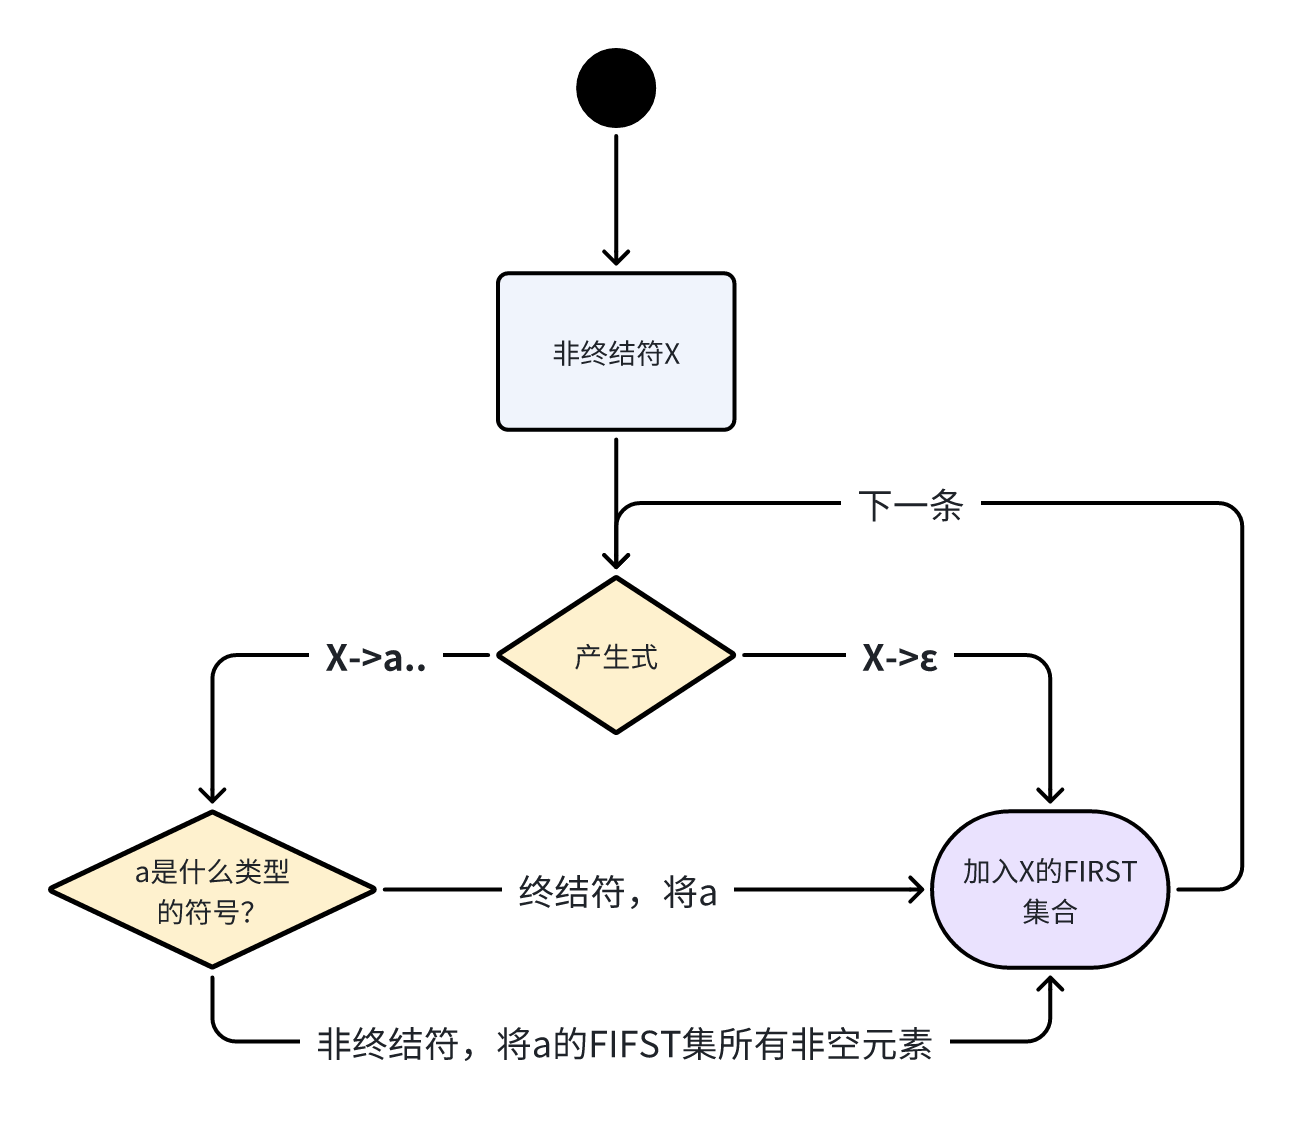
\includegraphics[width=0.8\linewidth]{assets/FIRST流程图.png}
\caption{求FIRST集合流程图}
\label{fig:求FIRST集合流程图}
\end{figure}

求FIRST集合的方法如图所示,在编译原理课程中已经详细学习过了,故在此不解释基本原理。代码中BuildFirstSet()即为求FIRST集合的方法,使用了一个变量changed来表示当前一次求闭包的过程有无增加新的元素,以此确定FIRST集合闭包是否已经生成成功。

\paragraph{求项目集的产生式闭包}
\begin{figure}[h]
\centering
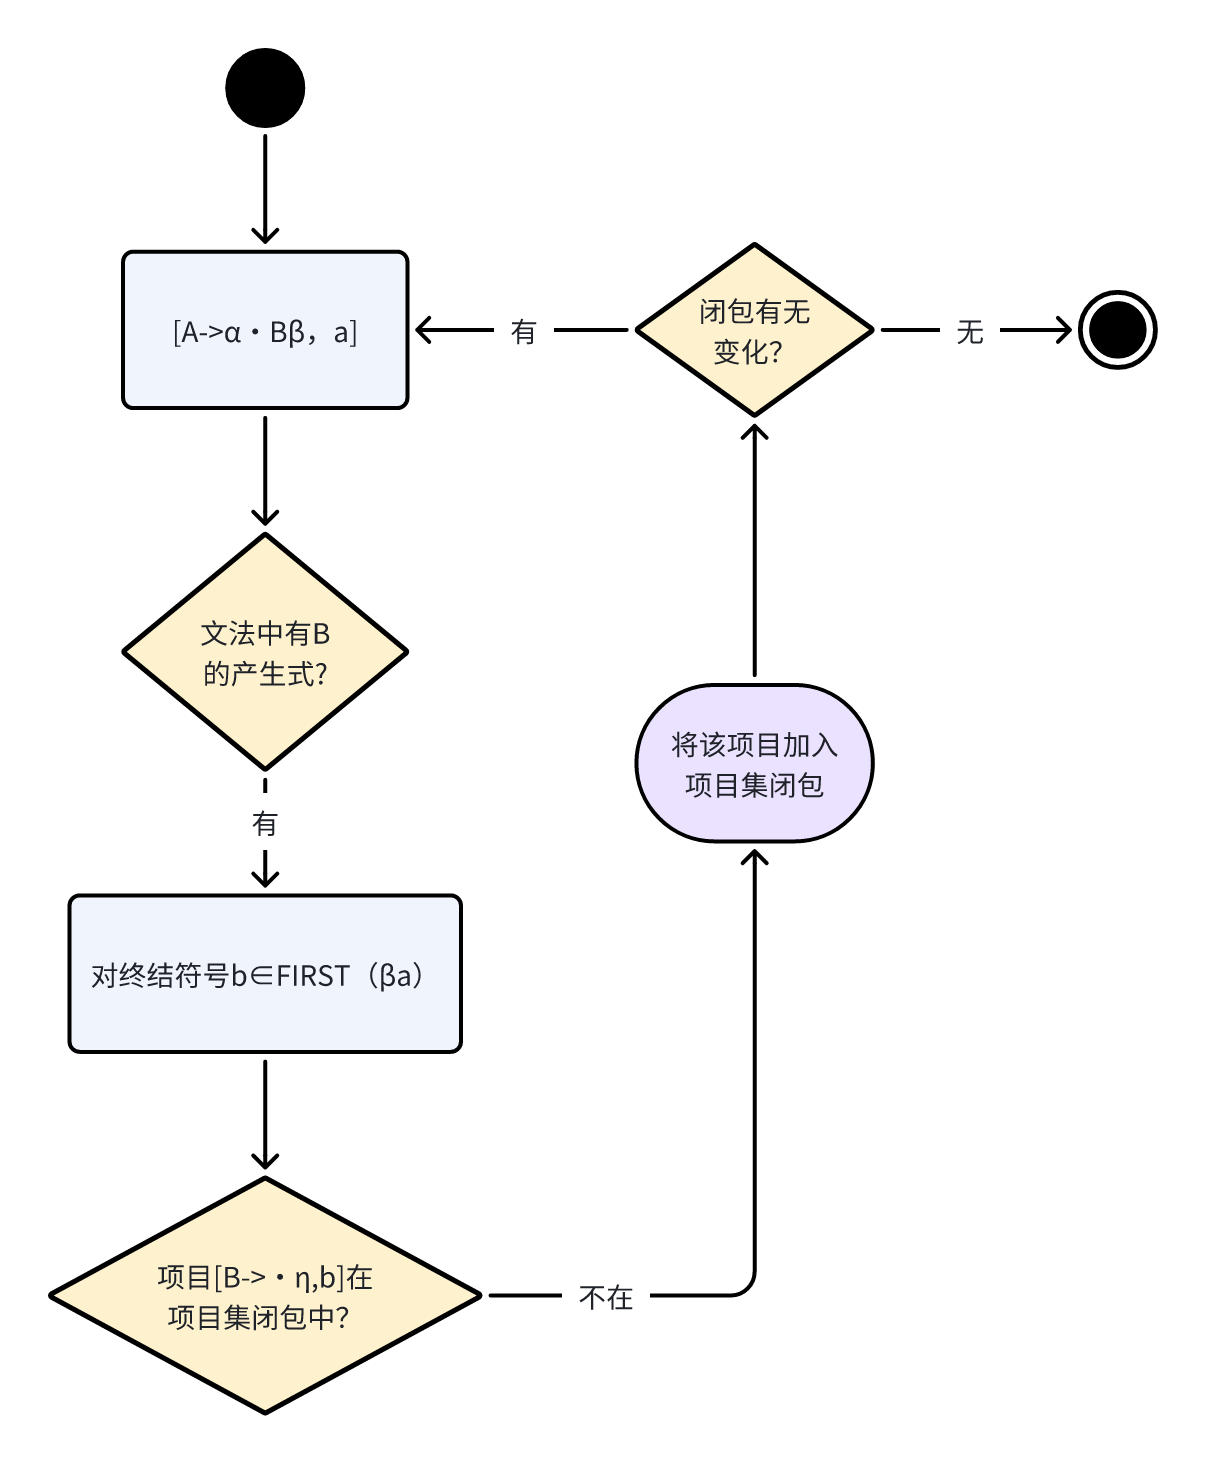
\includegraphics[width=0.5\linewidth]{assets/项目集闭包流程图.png}
\caption{求项目集产生式闭包流程图}
\label{fig:求项目集产生式闭包流程图}
\end{figure}

求项目集产生式闭包的方法如图所示。代码中CalculateClosure()即为对应方法。使用哈希值代表一个Expression,可以有效进行表达式的比较。

\paragraph{求DFA状态闭包}

\begin{figure}[htbp]
\centering
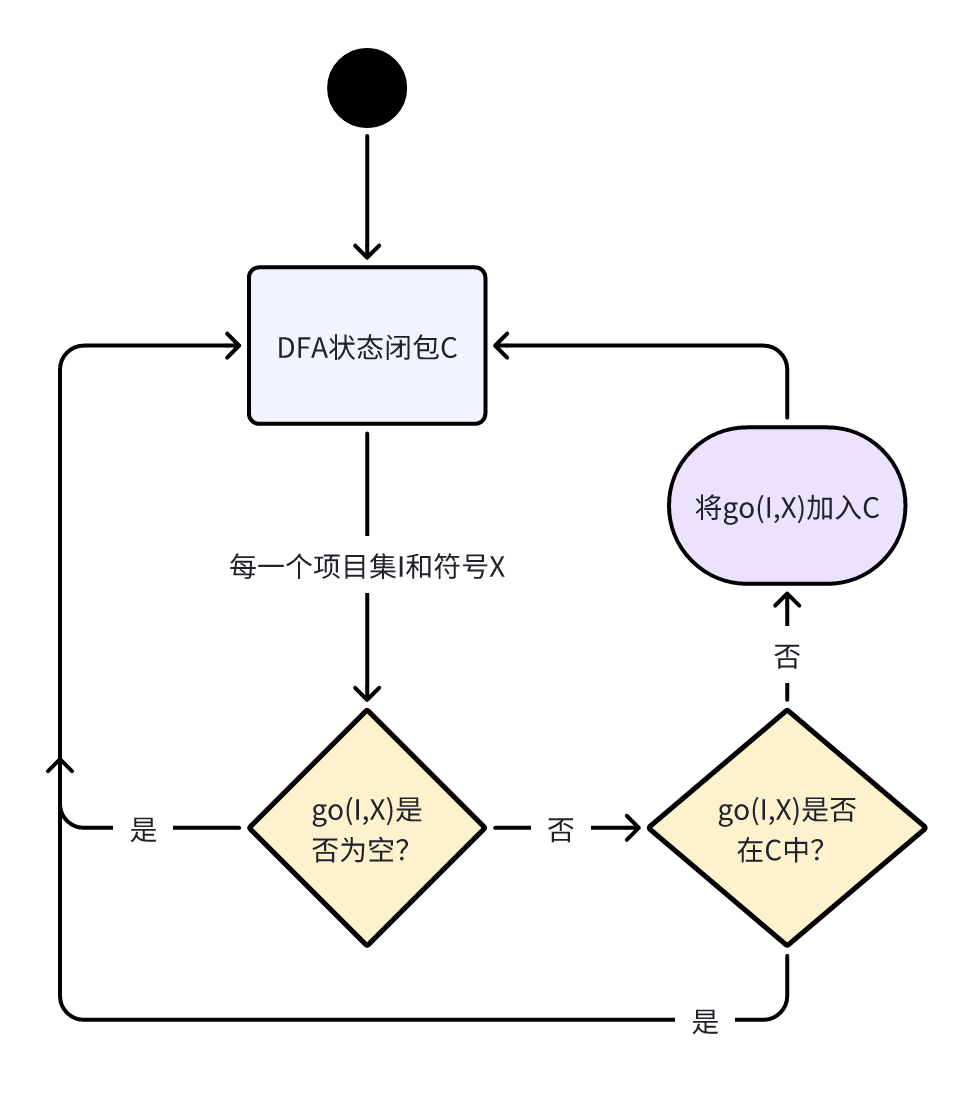
\includegraphics[width=0.5\linewidth]{assets/DFA状态闭包流程图.png}
\caption{求DFA状态集闭包流程图}
\label{fig:求DFA状态集闭包流程图}
\end{figure}

求DFA状态集闭包的方法如图所示。代码中Build()即为对应方法。

\paragraph{生成状态转移表}

状态转移表从DFA生成,可供记号流进行移进-归约而完成语法分析。
生成状态转移表的流程如下:
\begin{itemize}
    \item 构造文法G'的LR(1)项目集规范族C=\{$I_0$,$I_1$,...,$I_n$\},对于状态i(代表项目集$I_i$):
    \item 若[A→α·aβ,b]$\in$I, 且go(I,a)=$I_j$, 则置 action[i,a]=$S_j$
    \item 若[A→α·,a]$\in$I,且A不等于S',则置 action[i,a]=$R_j$
    \item 若[S'→S·,\$]$\in$I,则置 action[i,\$]=ACC
    \item 若对非终结符号A,有go($I_i$,A)=I,则置goto[i,A]=j
    \item 凡是不能用上述规则填入信息的空白表项,均抛出语法分析错误
\end{itemize}


\paragraph{生成语法树}

生成语法树实际上是利用DFA对输入记号流进行移进-归约的过程实现的。当从栈顶弹出符号时,就是向语法树子节点列表添加子节点的时候;当向栈压入符号时,就是整合子节点列表创建一个语法树父节点的时候;由于使用的是LR(1)自底向上的分析方法,因此最后生成的父节点就是分析器返回给编译程序的语法树根节点,由这个根节点便可以访问整棵语法树。

为了加快运行速度,减少生成语法树时重复建立转移表的时间,定义GeneratedTransformer类将转移表转换为可以外部保存的文件形式。编译器可通过读取文件直接载入转移表生成语法树,有效提高了运行效率。

\subsection{语义分析}

\subsubsection{核心数据结构}

\paragraph{Pascal类型系统}

为了在语法树上表示变量节点的类型,便于类型传递与检查,需要提供一个Pascal的类型系统。

\subparagraph{Pascal类型系统构成}
\begin{figure}[htbp]
\centering
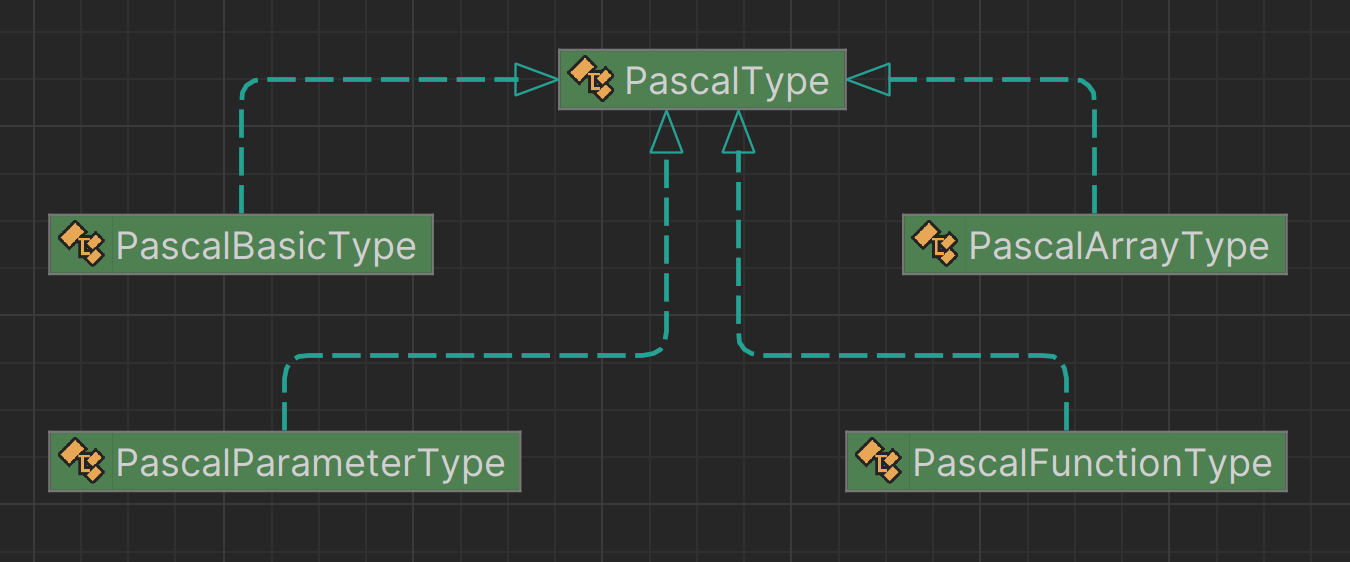
\includegraphics[width=0.5\linewidth]{assets/类型系统.png}
\caption{Pascal类型系统}
\label{fig:类型系统}
\end{figure}

\begin{itemize}
    \item \textbf{PascalType}类
作为类型系统基类,提供最基本的判等、转换类型、进行数学运算等功能。

\begin{lstlisting}[style=csharp]
    /// 类型的名称
    public abstract string TypeName { get; }

    /// 将当前类型转换为引用类型
    /// 原有类型变量保持不变
    /// 返回原有Pascal类型的引用类型
    public abstract PascalType ToReferenceType();

    /// 是否为引用类型
    public bool IsReference { get; init; }
\end{lstlisting}

\item \textbf{PascalBasicType}类
继承基类的Pascal基础类型,提供integer,boolean,char,real,void五种基础类型的单例对象。

\begin{lstlisting}[style=csharp]
    /// 整数类型的单例对象
    public static PascalType Integer => new PascalBasicType(BasicType.Integer);

    /// 布尔类型的单例对象
    public static PascalType Boolean => new PascalBasicType(BasicType.Boolean);

    /// 字符类型的单例对象
    public static PascalType Character => new PascalBasicType(BasicType.Character);

    /// 浮点数类型的单例对象
    public static PascalType Real => new PascalBasicType(BasicType.Real);

    /// 空类型的单例对象
    public static PascalType Void => new PascalBasicType(BasicType.Void);
\end{lstlisting}

\item \textbf{PascalArrayType}类
继承基类的Pascal数组类型,表示一个Pascal中的数组类型。

\begin{lstlisting}[style=csharp]
    // 数组元素的类型
    public PascalType ElementType { get; } = elementType;

    // 数组的起始范围
    public int Begin { get; } = begin;

    // 数组的结束范围
    public int End { get; } = end;

    // 数组的类型名
    public override string TypeName => $"{ElementType.TypeName}_{Begin}_{End}";
\end{lstlisting}

\item \textbf{PascalParameterType}类
继承基类的Pascal参数列表类型,用于过程等需要参数列表的场景。

\begin{lstlisting}[style=csharp]
    // 参数列表元素类型
    public PascalType ParameterType { get; } = parameterType;

    // 参数列表名称
    public string ParameterName { get; } = parameterName;

    // 参数列表的类型名
    public override string TypeName => $"{ParameterType}_{ParameterName}";
\end{lstlisting}
\end{itemize}


\paragraph{符号表类(SymbolTable)} 符号表类是编译器中用于存储变量与函数声明信息的数据结构,支持编译过程中的多种活动,如变量查找、类型检查和作用域控制,也用于代码生成时获取参数类型和值。

\subparagraph{符号表数据结构}
每个符号表类项包括:
\begin{itemize} 

    \item 符号表
    
    \begin{lstlisting}[style = csharp]
        Dictionary<string, Symbol> _symbols
    \end{lstlisting}

采用字典类型存储符号表内容。键为符号的名字,值为符号类型Symbol。

    \item 父符号表
    
    \begin{lstlisting}[style = csharp]
        private readonly SymbolTable? _parent;
    \end{lstlisting}

需要记录父符号表以便于重定位。

    \item 获得当前符号表的所有祖先符号表

    \begin{lstlisting}[style = csharp]
        public IEnumerable<SymbolTable> ParentTables => GetParents();
    \end{lstlisting}

用于在内部作用域查询外部变量信息。
    
\end{itemize}

\subparagraph{符号类(Symbol)} 符号类是一个Pascal符号在符号表中的存储对象,由类型检查在遍历语法树的过程中创建并存在在符号表中。

符号类的数据结构如下所示:
\begin{itemize}
    \item 符号名字
    
    \begin{lstlisting}[style = csharp]
        public required string SymbolName
    \end{lstlisting}
    
    \item 符号类型
    
    \begin{lstlisting}[style = csharp]
        public required PascalType SymbolType
    \end{lstlisting}

    \item 是否为常量
    
    \begin{lstlisting}[style = csharp]
        public bool Const
    \end{lstlisting}

\end{itemize}

\subparagraph{符号表的组织}
使用\texttt{栈式哈希符号表}管理不同作用域下的符号信息,通过链表实现了栈式结构的存储。使得每进入一个新的作用域就压入一个新的符号表,每退出一个作用域就弹出当前符号表,并通过parent属性回到父符号表中。

\subparagraph{操作定义}
\begin{itemize}
    \item \textbf{检索操作}:查找当前及外围作用域中的符号。

    \begin{lstlisting}[style = csharp]
        public bool TryGetSymbol(string name, [NotNullWhen(true)] out Symbol? symbol)
    {
        if (_symbols.TryGetValue(name, out symbol))
        {
            return true;
        }

        foreach (SymbolTable table in ParentTables)
        {
            if (table._symbols.TryGetValue(name, out symbol))
            {
                return true;
            }
        }

        symbol = null;
        return false;
    }
    \end{lstlisting}
    
    \item \textbf{插入操作}:在符号表中加入新的符号。

    \begin{lstlisting}[style = csharp]
        public bool TryAddSymbol(Symbol symbol) => _symbols.TryAdd(symbol.SymbolName, symbol);
    \end{lstlisting}
    
    \item \textbf{定位与重定位操作}:用于处理作用域的变化,如函数或块的进入和退出。

    以过程的定义节点Subprogram为例,进入Subprogram时:
    \begin{lstlisting}[style = csharp]
        public override void PreVisit(Subprogram subprogram)
    {
        base.PreVisit(subprogram);

        SymbolTable = SymbolTable.CreateChildTable(); // 创建子符号表并定位
    }
    \end{lstlisting}

    退出Subprogram时:
    \begin{lstlisting}[style = csharp]
        public override void PostVisit(Subprogram subprogram)
    {
        base.PostVisit(subprogram);

        if (!SymbolTable.TryGetParent(out SymbolTable? parent))
        {
            return;
        }

        SymbolTable = parent; // 重定位为父符号表
    }
    \end{lstlisting}
    
\end{itemize}

\subsubsection{核心功能说明}

语义分析模块的核心功能主要分为两个部分:类型检查和代码生成。在编译器的设计中,对于表达式进行类型检查是确保类型安全的重要部分,通过分析表达式中的操作符和操作数,编译器可以确定表达式是否符合语言的类型规则。代码生成则是编译环节的最后步骤,通过结合语法分析和类型检查中获得信息,结合目标语言的各种特征将源语言翻译对指针的目标语言。同时,在代码生成的环节中还需要考虑如何提供源语言中的核心库,例如Pascal中的各种输入和输出函数。

为了确保上述功能能够方便的实现,在该模块中实现上述功能的类都继承了语法树上的访问者\texttt{SyntaxNodeVisitor},该类提供了对于语法树进行访问的功能,避免在上述两个类重复的编写访问语法树的逻辑。

\subsubsection{类型检查的算法}
在编译器设计中,对表达式进行类型检查是确保类型安全和正确性的关键步骤。通过分析表达式中的操作符和操作数,编译器可以确定表达式是否符合语言的类型规则。

为每个非终结符号设定若干综合属性,这些属性由表达式的子部分递归地确定。即语法树的前后序访问操作,会将子树的相关属性向上传播,在上层节点的返回方法中进行检查。这种方法允许编译器在解析表达式时即时地检测和报告类型错误,同时尽可能地更早发现错误。

\texttt{ConstDeclaration}:const参数定义赋值。

\begin{lstlisting}[style=csharp]
ConstDeclaration -> id = ConstValue | ConstDeclaration ; id = ConstValue
\end{lstlisting}

ConstDeclaration是const参数定义赋值的非终结符记号,需要使用“向前看”的方法,提前向下获得ConstValue右式的实际值的类型并赋给ConstValue的类型属性。同时,尝试向符号表加入该常量符号。

\begin{figure}[h]
\centering
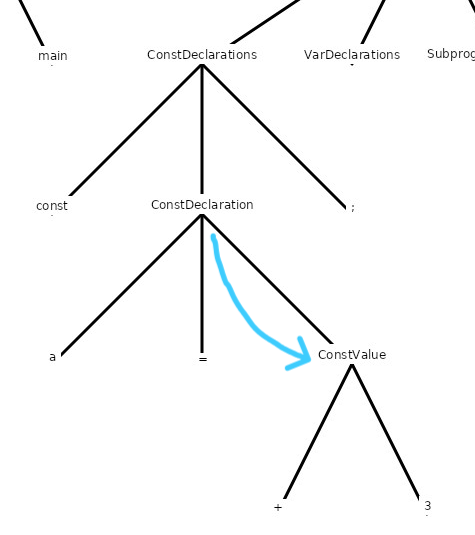
\includegraphics[width=0.4\linewidth]{assets/类型检查/constDeclaration.png}
\caption{ConstDeclaration的属性传递图}
\label{fig:ConstDeclaration}
\end{figure}

\texttt{Factor}:产生终结符或语句。

\begin{lstlisting}[style=grammar]
Factor -> num | Variable
         | ( Expression )
         | id ()
         | id (ExpressionList)
         | not Factor
         | - Factor
         | + Factor
         | true
         | false
\end{lstlisting}
        
Factor作为产生终结符和语句的上层,需要综合下层记号的类型,并向上传递。

\begin{figure}[h]
\centering
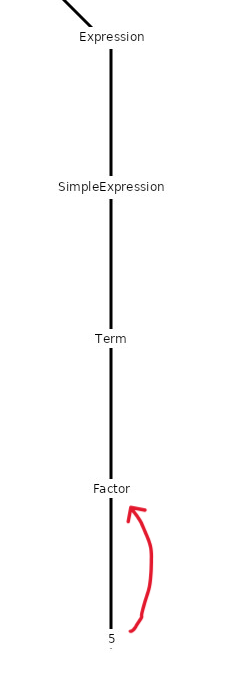
\includegraphics[width=0.2\linewidth ]{assets/类型检查/Factor.png}
\caption{Factor的属性传递图}
\label{fig:Factor}
\end{figure}

\texttt{Term}:产生含有Factor的表达式。

\begin{lstlisting}[style=grammar]
Term -> Factor | Term MultiplyOperator Factor
\end{lstlisting}

Term能够产生含有Factor的表达式,因此需要继续承接Factor表达式的类型并向上传递。同时,需要判断MultiplyOperator两侧的记号类型能否参与到运算中。
特别需要注意的是,不一定要求两侧的记号类型一致。如real和integer,会将计算结果赋予real类型。

\begin{figure}[h]
\centering
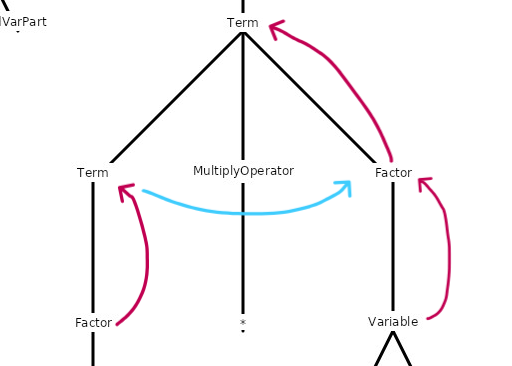
\includegraphics[width=0.5\linewidth ]{assets/类型检查/Term.png}
\caption{Term的属性传递图}
\label{fig:Term}
\end{figure}

\texttt{SimpleExpression}:产生含有Term的表达式。

\begin{lstlisting}[style=grammar]
SimpleExpression -> Term | SimpleExpression AddOperator Term
\end{lstlisting}

SimpleExpression能够产生含有Term的表达式,因此需要继续承接Term表达式的类型并向上传递。同时,需要判断AddOperator两侧的记号类型能否参与到运算中。

\textit{类型运算之后的结果由Pascal类型系统决定。}

\begin{figure}[h]
\centering
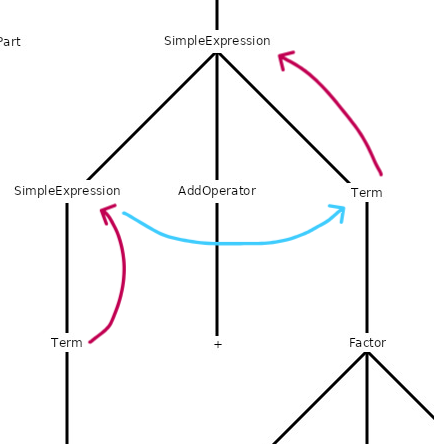
\includegraphics[width=0.5\linewidth ]{assets/类型检查/SimpleExpression.png}
\caption{SimpleExpression的属性传递图}
\label{fig:SimpleExpression}
\end{figure}

\texttt{Expression}:产生含有SimpleExpression的表达式。

\begin{lstlisting}[style=grammar]
Expression -> SimpleExpression | SimpleExpression RelationOperator SimpleExpression
\end{lstlisting}

Expression能够产生含有SimpleExpression的表达式,因此需要继续承接SimpleExpression表达式的类型并向上传递。对第二条产生式而言,由于Expression只会产生boolean RelationOperator boolean类型的表达式,故只需要返回boolean类型即可。

\begin{figure}[h]
\centering
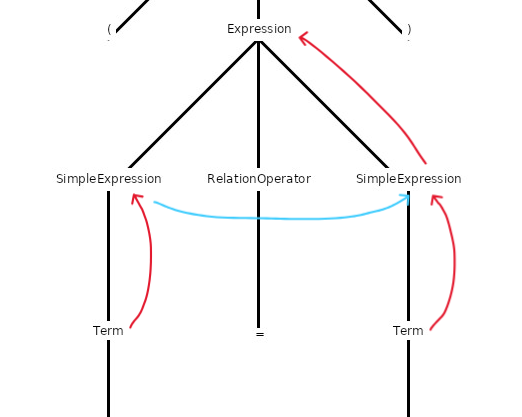
\includegraphics[width=0.5\linewidth ]{assets/类型检查/Expression.png}
\caption{Expression的属性传递图}
\label{fig:Expression}
\end{figure}

\texttt{TypeSyntaxNode}:指示记号类型的节点。

TypeSyntaxNode指示一个终结符类型。对于普通变量,将其类型直接赋予该节点类型即可。

对于数组需要特殊操作。of关键字后的类型将作为数组类型,但对于数组内部的各个维度的范围大小,需要逐层进行检查,以确保表示范围的两个参数均为integer。

\begin{figure}[h]
\centering
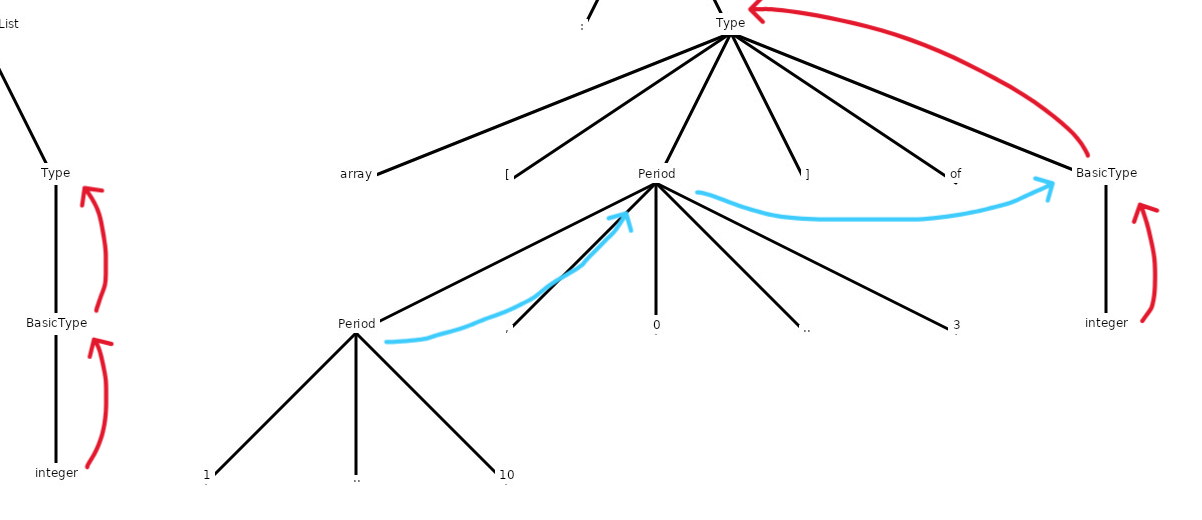
\includegraphics[width=0.8\linewidth ]{assets/类型检查/TypeSyntaxNode.png}
\caption{TypeSyntaxNode的属性传递图}
\label{fig:TypeSyntaxNode}
\end{figure}

\texttt{IdentifierList}:参数列表记号节点。

\begin{lstlisting}[style=grammar]
IdList -> , id IdList | : Type
\end{lstlisting}

IdentifierList指示一个产生如函数参数列表的列表记号。

这个参数列表的语法树构成如图\ref{fig:IdentifierList},为了区分引用类型和传值类型,需要在访问语法树进入该节点时将SubprogramHead中的IsReference和IsProcedure两个属性继承下来,前者表明这个列表是否为引用类型,通过有无关键字var确定;后者表明这个列表是否用于一个procedure的定义。

接下来,在返回过程中,要将从下层节点传上来的节点的类型与当前节点的这两个属性相匹配,生成新的符号放入符号表中。

\begin{figure}[htp]
\centering
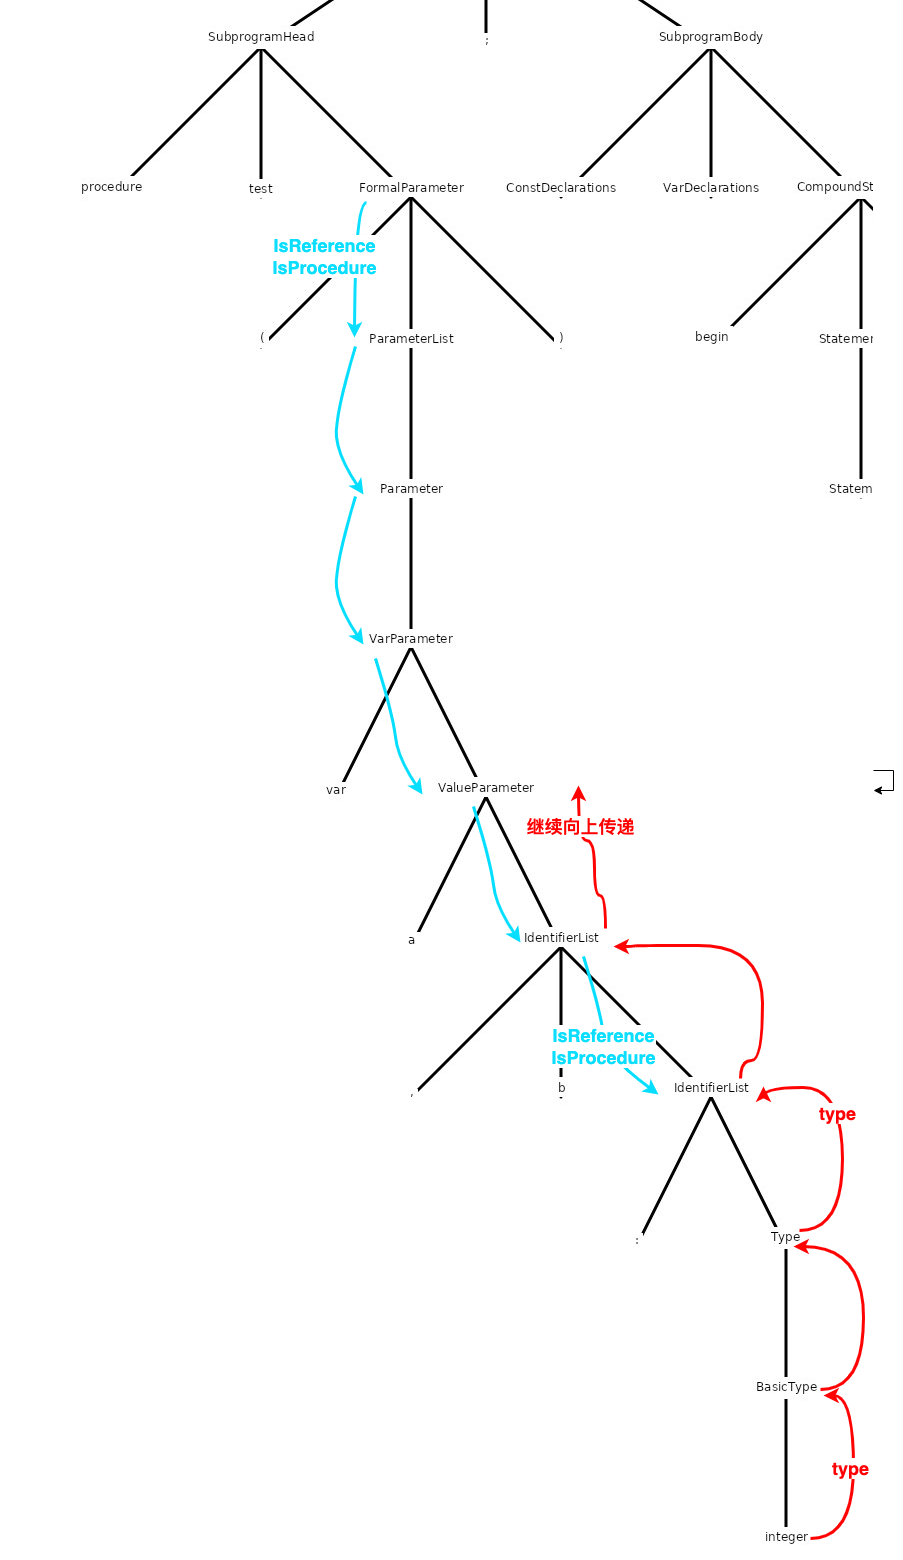
\includegraphics[width=0.8\linewidth ]{assets/类型检查/IdentifierList.png}
\caption{IdentifierList的属性传递图}
\label{fig:IdentifierList}
\end{figure}

\texttt{VarDeclaration}:变量列表记号节点。

\begin{lstlisting}[style=grammar]
IdList -> , id IdList | : Type
\end{lstlisting}

VarDeclaration指示一个产生如函数变量列表的列表记号。

在返回过程中,要将从下层节点传上来的节点的类型与当前节点的名字这两个属性相匹配,生成新的符号并作为作为一个列表记号放入符号表中。

\texttt{Subprogram}:过程节点。

\begin{lstlisting}[style=grammar]
Subprogram -> SubprogramHead ; SubprogramBody    
\end{lstlisting}

Subprogram负责作为过程定义的最上层节点。

在访问语法树进入该节点时,应当创建子符号表,以隔离内部变量。
在返回该节点时,应当修改当前符号表为父符号表,以还原符号表层级。

\begin{figure}[h]
\centering
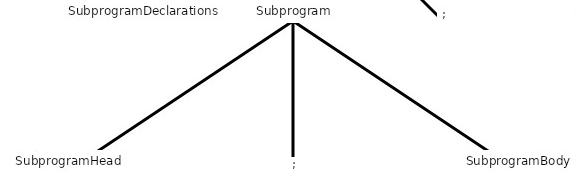
\includegraphics[width=0.8\linewidth ]{assets/类型检查/Subprogram.png}
\caption{Subprogram}
\label{fig:Subprogram}
\end{figure}

\texttt{SubprogramHead}:过程头节点。

\begin{lstlisting}[style=grammar]
SubprogramHead -> procedure id FormalParameter
                | function id FormalParameter : BasicType
\end{lstlisting}
                
SubprogramHead负责作为过程定义的头节点。

在访问语法树进入该节点时,应当重置参数表。

在返回该节点时,应当向父符号表加入该过程id和其所需参数。如果存在返回值,应当向符号表加入同过程名的返回值类型的变量,表示过程运算结果。

观察语法树(图\ref{fig:IdentifierList}),可以注意到参数列表中每个参数的位置实际上与真实位置恰好相反,这主要是因为语法树中靠前的参数在上层,在返回节点收集参数时靠后收集,故需要通过一定的操作将参数列表反转。又因为参数列表由多个不同变量类型的变量列表构成,因此定义一个二维数组,每一行表示一种类型的变量列表,只需要在参数列表中反转这个二维数组即可。

\begin{figure}[h]
\centering
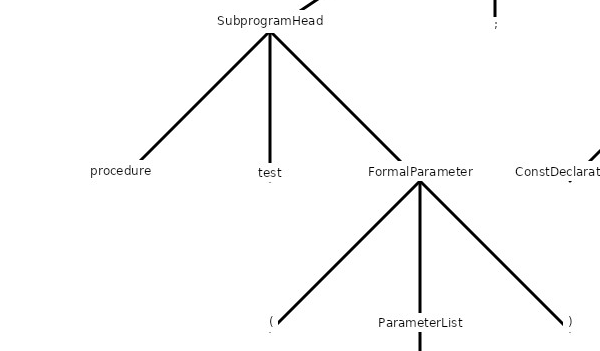
\includegraphics[width=0.8\linewidth ]{assets/类型检查/SubprogramHead.png}
\caption{SubprogramHead}
\label{fig:SubprogramHead}
\end{figure}

\texttt{VarParameter}:引用变量列表。

\begin{lstlisting}[style=grammar]
VarParameter -> var ValueParameter
\end{lstlisting}

VarParameter负责定义引用变量列表。

在访问语法树进入该节点时,应当创建一个引用变量列表。
由于引用变量列表实际上就是通过包装一个变量列表,将其IsReference设为true来实现,故这个节点只实现包装功能。

\texttt{ValueParameter}:变量列表。

\begin{lstlisting}[style=grammar]
ValueParameter -> id IdList
\end{lstlisting}

ValueParameter负责定义变量列表。

在访问语法树进入该节点时,应当创建一个变量列表。

在返回过程中退出该节点时,应当向符号表内加入参数符号,同时向参数列表加入该符号,供上层的VarParameter节点使用。

\texttt{Statement}:句子节点,能够产生不同类型的句子,代码检查阶段需要检查这些句子。

\begin{itemize}
    \item 对于空产生式无需检查
    
    \begin{lstlisting}[style=grammar]
        Statement -> $\epsilon$
    \end{lstlisting}
    
    \item 通过在符号表中搜索符号,检查是否定义变量。通过检查符号是否为常量,检查变量能否被再赋值。通过判等变量与表达式的类型,检查变量能否被右侧表达式结果赋值。

    \begin{lstlisting}[style=grammar]
        Statement -> Variable AssignOp Expression
    \end{lstlisting}
    
    \item 对于这个产生式无需检查,相关的类型检查由函数调用的节点负责进行。

    \begin{lstlisting}[style=grammar]
        Statement -> ProcedureCall
    \end{lstlisting}
    
    \item 对于这个产生式无需检查。

    \begin{lstlisting}[style=grammar]
        Statement -> CompoundStatement
    \end{lstlisting}
    
    \item 检查If语句的条件语句Expression是否为boolean。

    \begin{lstlisting}[style=grammar]
        Statement -> Statement -> if Expression then Statement ElsePart
    \end{lstlisting}
    
    \item 通过在符号表中搜索符号,检查是否定义循环变量,通过检查起始表达式类型,判断循环起始是否为整数,通过检查终结表达式类型,判断循环终结是否为整数。 
    
    \begin{lstlisting}[style=grammar]
        Statement -> for id AssignOp Expression to Expression do Statement
    \end{lstlisting}
    
    \item 检查While循环语句的条件变量Expression是否为boolean。

    \begin{lstlisting}[style=grammar]
        Statement -> while Expression do Statement
    \end{lstlisting}
\end{itemize}

\texttt{ProcedureCall}:调用过程

编译器将Procedure和Function均视为Procedure,区别在于Procedure不需要参数,而Function需要参数。为此,需要在调用过程区分是否需要参数。

在访问语法树退出该节点时,需要进行类型检查。

\begin{itemize}
    \item 通过在符号表中搜索符号,检查该过程是否定义
    \item 递归判断该符号类型,检查该符号是否能被调用
    \item 通过判断符号内的参数个数属性,检查调用过程时填入的参数个数是否与定义时的参数个数相同
    \item 通过判断符号内的参数类型属性,检查调用过程时填入的参数个数是否与定义时的参数类型相同    
\end{itemize}

同时,需要将过程的返回值类型赋给过程类型自身,便于上层节点获取。

\texttt{Variable}:变量产生节点。

\begin{lstlisting}[style=grammar]
Variable -> id IdVarPart
\end{lstlisting}

Variable负责定义产生一个变量。

在返回过程中退出该节点时,应当在符号表中查找这个符号,以确定这个符号已经声明。同时,应获取这个符号的类型并赋给自身的类型属性,便于向上传递变量引用时的类型。

若变量为数组类型,则需要利用IdVarPart的综合属性IndexCount,以检查实际赋值时变量维数与定义时维数是否一致。

\texttt{IdVarPart}:数组变量下标节点。

\begin{lstlisting}[style=grammar]
IdVarPart -> $\epsilon$ | [ ExpressionList ]
\end{lstlisting}

IdVarPart表示了数组变量的一个元素,如arr[1][1][4]。

在语法树访问退出该节点时,需要检查元素下标的每一维是否为integer类型。同时,需要将实际赋值时这个变量的维数作为综合属性IndexCount向上传递,在Varibale中完成进一步的类型检查。

\begin{figure}[htbp]
\centering
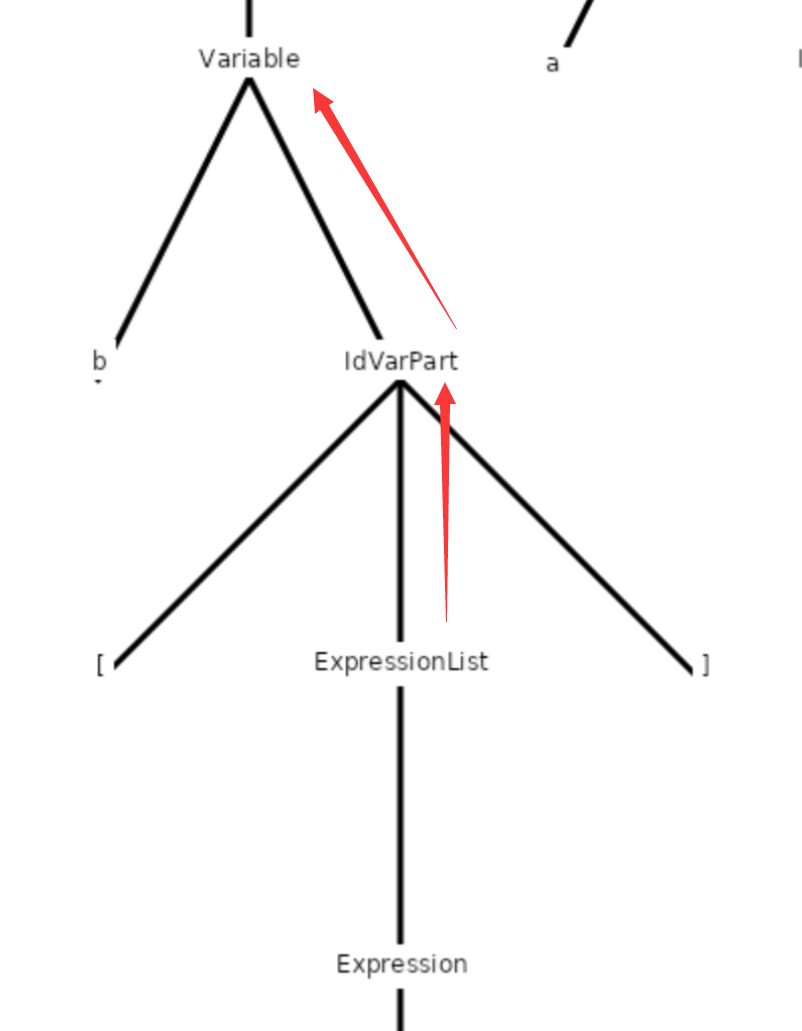
\includegraphics[width=0.8\linewidth ]{assets/类型检查/IdVarPart.png}
\caption{Variable与IdVarPart}
\label{fig:Variable与IdVarPart}
\end{figure}

\subsubsection{代码生成的算法}
代码生成是本次编译程序的最终阶段,利用语法树、类型检查阶段得到的信息和符号表,实现pascal代码到C代码的翻译。

\paragraph{设计思路}
为非终结符号和终结符号设定若干综合属性和继承属性。在前序遍历到某个语法树节点时,子节点继承属性完成初始化;在后序遍历回到这个语法树节点时,通过子节点的属性计算出该节点的综合属性。在遍历语法树的过程中,利用这些属性信息生成对应的C代码。

\paragraph{映射关系}

\begin{itemize}
    \item \textbf{头文件}
    
    Pascal-S用于输入的read、readln和用于输出的write、writeln分别对应于C程序的scanf和printf,因此需要加入stdio.h头文件。
    
    Pascal-S中的基本类型boolean,对应于C语言的bool,但bool不是C语言的基本类型,因此需要加入stdbool.h头文件。

    \item \textbf{常量和变量}
    
    Pascal-S中的常量和变量定义对应于C程序的全局常量和全局变量定义。

    \item \textbf{主程序定义}
    
    Pascal-S中的主程序可以为任意合法命名,而C语言的主程序名只能为main,因此将Pascal-S主程序名直接翻译为main即可。

    此外,Pascal的主程序头还可以包含一个参数列表,这个标识符列表对应于C语言中main函数的参数列表,但是由于Pascal-S缺少响应的库程序支持,因此主程序参数没有任何用途,所以在代码生成阶段,将忽略主程序的参数列表。
    
    \item \textbf{子程序声明}
    
    Pascal-S有procedure和function两种子程序,其中function直接对应于C语言的函数,procedure无返回值,对应于C程序中返回值为void类型的函数。

    \item \textbf{引用传参}
    
    Pascal-S中参数列表里带有var声明的为引用传参,对应于C语言中的指针。

    \item \textbf{函数/过程调用}
    
    Pascal-S中,不带参数的函数/过程可以不带括号调用,比如func()和func这两种调用方式均可,但C语言中,即使函数/过程调用不含参数,也必须使用一对空括号。

    此外,在引用传参时,还要在参数前添加取地址符'\&'。

    \item \textbf{返回语句}
    
    Pascal-S的返回语句是通过给函数名赋值来实现的,对应于C语言中需要用到return。
    
    \item \textbf{类型关键字}
    \begin{table}[h]
        \centering
        \begin{tabular}{|c|c|}
        \hline
        \textbf{Pascal-S关键字} & \textbf{C语言关键字}\\
        \hline
        integer & int\\
        \hline
        real & double\\
        \hline
        char & char\\
        \hline
        boolean & bool\\
        \hline
        \end{tabular}
    \end{table}

    \item \textbf{运算符}
    
    \begin{longtable}{|c|c|c|}
    \hline
    \textbf{运算符} & \textbf{Pascal-S} & \textbf{C语言}\\
    \hline
    \endhead
    \hline
    \multicolumn{3}{r@{}}{接下一页}
    \endfoot
    \hline
    \endlastfoot
    加 & + & + \\
    \hline
    减 & - & - \\
    \hline
    乘 & * & * \\
    \hline
    除 & / & / \\
    \hline
    整除 & div & / \\
    \hline
    取余 & mod & \% \\
    \hline
    与 & and & \&\& \\
    \hline
    或 & or & || \\
    \hline
    非 & not & \~{} \\
    \hline
    大于 & > & > \\
    \hline
    小于 & < & < \\
    \hline
    大于等于 & >= & >= \\
    \hline
    小于等于 & <= & <= \\
    \hline
    等于 & = & == \\
    \hline
    不等于 & <> & != \\
    \hline
    赋值 & := & = \\
    \hline
    \end{longtable}

    \item \textbf{数组}
    
    \textbf{数组下标 } 
    Pascal-S中数组上下标均可自定义,数组左边界不必从0开始;但是在C语言中,只能指定数组的上界,下界固定为0。因此我们用Pascal数组的每一维减去当前维度的左边界,将其映射为C语言的数组下标形式。

    \textbf{数组引用方式 }
    在Pascal-S中,数组的下标引用用一对中括号包裹,每一位维下标之间用逗号分隔。C语言中数组每一维下标都要用中括号包裹。
    此外,在引用数组元素时,每一个下标都要减去当前维度的左边界

    \item \textbf{复合语句}
    
    Pascal-S中符合语句是以begin关键字开始,end关键字结束,对应C语言中一对大括号包括。
    在Pascal-S中,复合语句的最后一条语句是没有分号的,而C语言中每条语句必须以分号结束。

    \item \textbf{赋值语句}
    
    Pascal-S中常量初始化的赋值语句和C语言一样,都是使用'='符号;而变量赋值时,Pascal-S采用':=',C语言采用'='。

    \item \textbf{表达式}
    
    将表达式翻译为三地址代码的形式。
    
    \item \textbf{分支语句和循环语句}
    
    统一翻译为C语言的goto语句。

    \item \textbf{输入输出语句}
    
    Pascal-S在使用read/readln和write/writeln进行输入输出时,将变量作为参数传递即可。而C语言中的scanf和printf函数不仅要传入变量,还需要声明格式化字符串。
    
\end{itemize}

\paragraph{具体实现}
\begin{itemize}
    \item \textbf{头文件的输出}
    
    在前序遍历到programHead时就将stdio.h和stdbool.h两个头文件定义输出。
    输出格式:
    \begin{lstlisting}[style = c]
        #include <stdio.h>
        #include <stdbool.h>
    \end{lstlisting}

    \item \textbf{全局常量的输出}
    
    在后序遍历到constDeclaration时,从节点中获取常量名和常量值,从符号表里获取常量的类型。输出格式:
    \begin{lstlisting}[style = c]
        const 常量类型 常量名 = 常量值;   
    \end{lstlisting}

    \item \textbf{全局变量的输出}
    
    变量定义的相关信息存储在了varDeclaration节点的IdList里,于是可以在后序遍历回到IdList时直接从节点里取出类型,标识符名;将类型解析成C语言形式的类型之后,按照如下格式输出:
    \begin{lstlisting}[style = c]
        变量类型 变量名;  
    \end{lstlisting}

    由于变量定义用到的IdList -> id,IdList 是一个右递归,而每次是后序遍历到varDeclaration时才生成一个变量定义。因此,得到的C代码的变量列表实际上与Pascal的变量列表顺序是相反的,但这并不影响程序的逻辑。

    对于数组类型的变量定义输出格式为:
    \begin{lstlisting}[style = c]
        数组元素类型 数组名 [维度1][维度2][维度3]...... ;
    \end{lstlisting}

    \item \textbf{子函数头的输出}
    
    在后序遍历到subprogramHead时,符号表里已经插入了子函数头的相关定义,于是可以直接从符号表里获取函数的返回类型(如果是procedure,返回类型为void)。

    接下来是生成参数列表。虽然参数列表的定义里用到了Idlist,但是由于IdList的后序遍历输出的变量列表与定义时的顺序相反,因此不能直接在IdList的后序遍历方法中输出参数列表,函数的参数列表定义必须严格保持其原先的顺序。此时可以直接从函数的类型里将参数列表取出,然后按照[类型] [参数名] 的格式依次输出每一个参数定义即可,参数之间用逗号分隔。(传参是否为引用的判断已经封装在了类型解析里)

    子函数头的输出格式:
    \begin{lstlisting}[style = c]
        返回值类型 函数名 ( 参数列表 )
    \end{lstlisting}
    
    \item \textbf{函数体的输出}
    
    Pascal-S中函数体用一个compoundStatement表示,于是在前序遍历到compoundStatement的时候开启一段代码块,输出左大括号;在后序遍历到compoundStatement的时候结束一段代码块,输出右大括号。这一对大括号构成C语言函数体最外层的大括号。

    \item \textbf{表达式的输出}
    
    为了方便后续翻译分支语句和循环语句等,涉及到表达式的语句将会以被翻译成三地址代码的形式。

    \textbf{三地址代码的生成}
    
    观察图\ref{fig:赋值语句的翻译},可以清晰地看到三地址代码的产生过程。在变量没有进行运算时,会直接向上层传递;而每当变量进行一次运算,就会产生一个新的临时变量来存储计算结果(此时会输出这个临时变量的赋值表达式),然后将这个临时变量向上层传递。当传递到statement的时候,整个赋值语句翻译完毕。

    \begin{lstlisting}[style = c]
        //翻译前 
        a := a + b * c;

        //翻译后
        int __temp_0 = b * c;
        int __temp_1 = a + __temp_0;
        a = __temp_1;
    \end{lstlisting}
    
    \begin{figure}[htbp]
        \centering
        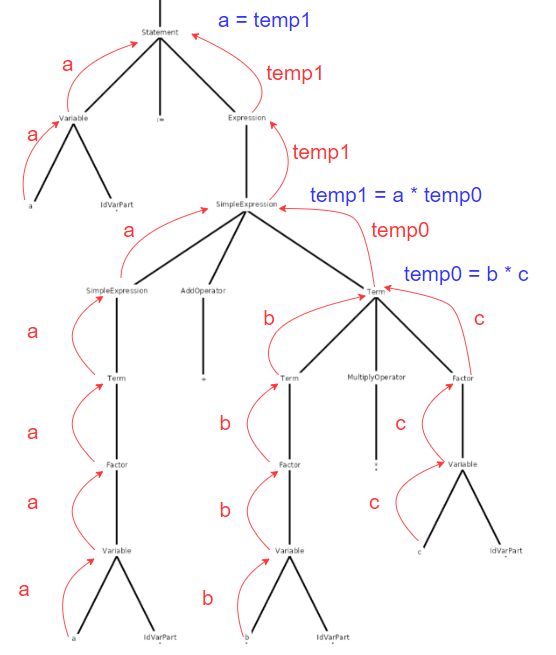
\includegraphics{assets/代码生成/赋值语句的翻译.png}
        \caption{赋值语句的翻译}
        \label{fig:赋值语句的翻译}
    \end{figure}


    \item \textbf{if语句的翻译}

    对于if语句的代码生成,需要用到如下辅助栈:
    \begin{lstlisting}[style = csharp]
    /// <summary>
    /// 存储IF语句中条件变量的名称
    /// </summary>
    private readonly Stack<string> _ifConditionNames = new();

    /// <summary>
    /// IF语句中成功分支的标签
    /// </summary>
    private readonly Stack<string> _ifTrueLabels = new();

    /// <summary>
    /// IF语句中失败分支的标签
    /// </summary>
    private readonly Stack<string> _ifFalseLabels = new();

    /// <summary>
    /// IF语句中结束的标签
    /// </summary>
    private readonly Stack<string> _ifEndLabels = new();   
    \end{lstlisting}

    \textbf{必要信息入栈}
    
    在后序遍历到expression时,将expression的变量名压入\_ifConditionNames栈中;
    在遍历到终结符'then'时,产生翻译if语句需要的三个标签,并压入对应标签栈中。

    \textbf{使用栈中的属性}

    当遍历到终结符'then'时,取变量栈栈顶的条件变量名,和相应标签栈栈顶的标签名,按照如下格式输出:
    \begin{lstlisting}[style = c]
        if (条件变量名) 
            goto 分支成功标签;
        else 
            goto 分支失败标签;
        分支成功标签:;
    \end{lstlisting}

    当前序遍历到elsePart节点时,由于成功分支不再执行else中的代码,于是需要在此处先输出goto语句,使其跳转到if结束标签处。接着,输出分支失败标签,表示接下来是else的代码段。输出格式如下:
    \begin{lstlisting}[style = c]
        goto 分支结束标签;
        分支失败标签:;
    \end{lstlisting}

    当后序遍历到elsePart节点时,输出分支结束标签,并将涉及到的变量栈和标签栈栈顶弹出,标志分支翻译结束。输出代码格式如下:
    \begin{lstlisting}[style = c]
        分支结束标签:;
    \end{lstlisting}

    \textbf{使用栈存储的原因 } 解决嵌套结构的if语句。
    
    \item \textbf{for循环的翻译}
    
    为了简化翻译的逻辑,将for循环翻译为条件分支if语句和goto语句的组合。
    
    在翻译过程需要用到如下辅助栈:

    \begin{lstlisting}[style = csharp]
     /// <summary>
    /// FOR语句中的循环变量名称
    /// </summary>
    private readonly Stack<string> _forVariables = new();
    
    /// <summary>
    /// FOR语句中的循环变量的初始值
    /// </summary>
    private readonly Stack<string> _forBeginConditions = new();
    
    /// <summary>
    /// FOR语句中循环变量的判断值
    /// </summary>
    private readonly Stack<string> _forEndConditions = new();
    
    /// <summary>
    /// FOR语句开始的标签
    /// </summary>
    private readonly Stack<string> _forLabels = new();
    
    /// <summary>
    /// FOR语句条件判断部分的标签
    /// </summary>
    private readonly Stack<string> _forConditionLabels = new();
    
    /// <summary>
    /// FOR语句结束的标签
    /// </summary>
    private readonly Stack<string> _forEndLabels = new();       
    \end{lstlisting}

    \textbf{必要信息入栈供翻译使用}
    
    在前序遍历到statement时,如果是for循环语句,将循环变量的变量名名压入\_forVariable栈中;在后序遍历到expression时,如果当前表达式是for循环的循环变量赋初值的表达式,则将expression节点中的变量名压入\_forBeginConditions栈中;如果当前表达式是for循环的边界条件,则将expression节点中的变量名压入\_forEndConditions栈中。

    \textbf{使用栈中的信息 }
    
    在后序遍历到终结符节点'to'时,当前for循环的循环变量及其初值变量必然位于对应栈的栈顶,此时输出循环变量赋初值的C代码,格式为 [循环变量名] = [循环变量初值变量]。此时还应产生for循环要用到的三个标签,并压入栈中,分别为:for循环的条件标签,for循环的主体标签,for循环的结束标签。此时输出for循环的条件标签,表示接下来的内容为条件判断部分。输出格式为:

    \begin{lstlisting}[style = c]
        循环变量名 = 初值变量;
        for循环条件标签:;
    \end{lstlisting}

    在后序遍历到终结符节点'do'时,当前for循环的边界条件变量位于\_forEndConditions栈的栈顶。此时输出条件判断部分,此外还应输出for循环主体标签,表示接下来的内容为for循环主体。输出格式:

    \begin{lstlisting}[style = c]
        if ( 循环变量 <= 边界变量 ) 
            goto for循环主体标签;
        else 
            goto for循环结束标签
        for循环主体标签:;
    \end{lstlisting}

    在后序遍历回到产生for循环的statement节点时,输出更新循环变量的C语言语句,并用goto语句跳转到条件判断标签处(这一步是实现“循环”的关键)。接着,输出for循环结束标签,将对应变量栈和标签栈的栈顶弹出,标志for循环翻译完毕。
    输出格式:
    \begin{lstlisting}[style = c]
        循环变量 = 循环变量 + 1;
        goto for循环条件标签;
        for循环结束标签:;
    \end{lstlisting}

    \item \textbf{while循环的翻译}
    
    与for循环类似,将while语句也翻译为条件分支if语句和goto语句的组合。

    此时要用到的辅助栈如下:
    \begin{lstlisting}[style = csharp]
    /// <summary>
    /// WHILE语句条件变量的标签
    /// </summary>
    private readonly Stack<string> _whileConditionNames = new();

    /// <summary>
    /// WHILE语句开始的标签
    /// </summary>
    private readonly Stack<string> _whileBeginLabels = new();

    /// <summary>
    /// WHILE语句结束的标签
    /// </summary>
    private readonly Stack<string> _whileEndLabels = new();    
    \end{lstlisting}

    在先序遍历到expression节点时,产生while循环要用到的三个标签并压入栈中。此时输出while循环条件标签,表示接下来的程序段为while循环条件判断,输出格式如下:
    \begin{lstlisting}[style = c]
        while循环条件标签:;    
    \end{lstlisting}

    在后序遍历到终结符节点'do'时,输出while条件判断内容,格式如下:
    \begin{lstlisting}[style = c]
        if(while条件变量 == false)
            goto while结束标签;
    \end{lstlisting}

    在后序遍历到产生while语句的statement节点时,输出goto语句跳转到while条件判断标签处。接着,输出while循环结束标签,并将对应变量栈和标签栈弹出,while循环翻译完毕。输出格式:
    \begin{lstlisting}[style = c]
        goto while循环条件标签;
        while循环结束标签:;
    \end{lstlisting}
    
    \item \textbf{函数/过程调用的翻译}
    
    由于Factor和ProcedureCall都能够产生函数/过程调用语句,因此在后序遍历回到这两个节点时,都要生成函数调用的代码。

    对于引用传递的参数,需要在输出的参数前添加取地址符'\&'。此外,还需要特殊处理函数内部的递归。

    输出格式:
    \begin{lstlisting}[style = c]
        函数名( 参数1, 参数2......)
    \end{lstlisting}

    \item \textbf{输入输出语句的翻译}

    输入输出语句会被当作普通的函数调用语句来处理,但是区别是需要在参数列表之前添加格式化字符串。此外,在scanf的参数列表中,每一个参数前需要添加取地址符'\&'。格式如下:
    \begin{lstlisting}[style = c]
        //输入
        scanf("%d", &a)
        //输出
        printf("%d", a) 
    \end{lstlisting}

    \item \textbf{main函数的翻译}

    main函数生成的位置其实和Pascal-S主程序体的位置是一样的,但是需要在适当的时机生成main函数头和main函数的返回语句。

    由于每一个函数体都对应一个compoundStatement,于是我们在该节点上设置属性IsMain,在先序遍历到programBody时将主程序体对应的compoundStatement的IsMain设置为true。在先序遍历到compoundStatement时,生成main函数头,格式为:
    \begin{lstlisting}[style = c]
        int main() 
    \end{lstlisting}
    在后序遍历回到compoundStatement节点时,如果IsMain为true,生成main函数返回语句,输出格式:
    \begin{lstlisting}[style = c]
        return 0;
    \end{lstlisting}
    
    \item \textbf{处理短路问}
    对于布尔表达式,需要处理短路的问题,主要是针对and和or操作。需要用到的辅助数据结构如下:
    \begin{lstlisting}[style = csharp]
    
    private record CircuitLabel(string Circuit, string End);

    private readonly Stack<CircuitLabel> _andCircuitLabels = [];

    private readonly Stack<CircuitLabel> _orCircuitLabels = [];    
    \end{lstlisting}

    \textbf{and的短路}

    在后序遍历到终结符'and'时,取and左侧变量名,取\_andCircuitLabels栈中的and短路标签,输出格式:
    \begin{lstlisting}[style = c]
        if(!左侧变量名)
            goto 短路标签;   //如果and左操作数为false,则无需判断右操作数
    \end{lstlisting}

    在后序遍历到term节点时,输出如下C代码:
    \begin{lstlisting}[style = c]
        bool temp = 左侧变量 && 右侧变量; //执行与操作
        goto 短路结束标签;    //跳过短路代码段
        短路标签:;
        temp = false;   //被短路时,直接设置条件为false
        短路结束标签:;
    \end{lstlisting}

    \textbf{or的短路}

    在后序遍历到终结符'or'时,取or左侧变量,取\_orCircuitLabels栈顶的短路标签,按如下格式输出:
    \begin{lstlisting}[style = c]
        if(左侧变量名)
            goto 短路标签;   //如果or左操作数为true,则无需判断右操作数
    \end{lstlisting}

    在后序遍历到simpleExpression节点时,输出如下C代码:
    \begin{lstlisting}[style = c]
        bool temp = 左侧变量 or 右侧变量; //执行或操作
        goto 短路结束标签;    //跳过短路代码段
        短路标签:;
        temp = true;   //被短路时,直接设置条件为true
        短路结束标签:;
    \end{lstlisting}
    
\end{itemize}

\end{document}